\chapter{ННК GaN: влияние подготовки поверхности Si на морфологию и оптические
свойства}\label{ch:ch4}

В данной главе излагается результат исследования влияния подготовки поверхности
подложки Si(111) и состава буферного слоя на морфологию и оптические свойства
ННК GaN, синтезированных методом ПА-МПЭ. Изучено формирования ННК GaN на
подложке Si(111) с промежуточным слоем SiN\textsubscript{x}, затравочными
островками AlN, буферными слоями GaO\textsubscript{x}, субмонослойными
смачивающими слоями Ga и затравочным островками GaN.

Образование вертикально ориентированных ННК GaN показано на подложках Si(111) и
Si(100) \cite{Corfdir2009}. В обоих случаях ННК GaN имеет кристаллическую
структуру WZ с направлением роста вдоль нормально ориентированной к поверхности
подложки оси с. ННК на Si(100) имеют две возможных ориентаций ННК в плоскости
из-за разницы в симметрии плоскостей (001)\textsubscript{Si} и
(0001)\textsubscript{GaN} \cite{Largeau2008}.

Одним из основных недостатков синтеза ННК GaN на подложке Si~--- это
образование нанометровой прослойки аморфного нитрида кремния на гетерогранице
GaN/Si из-за разницы между энергиями связи Si-N~(4,5~\si{\electronvolt}) и
Ga-N~(2,2~\si{\electronvolt}) \cite{Stoica2008}. Такой промежуточный слой с
широкой запрещённой зоной неизбежно ограничивает приборное применение, создавая
барьер для носителей заряда.

В работе \cite{Stoica2008} показано, что вертикально ориентированные массивы
ННК GaN с высоким качеством кристаллической структуры могут быть выращены даже
на некристаллической поверхности: рост на термически оксидированной подложке
Si(100), покрытой слоем аморфного SiO\textsubscript{2} толщиной \(\approx
320\)~\si{\nano\meter} приводит к образованию случайным образом ориентированных
в плоскости вертикальных WZ-GaN ННК.  Также сообщалось о росте ННК GaN на
аморфном слое Al\textsubscript{x}O\textsubscript{y} толщиной
15~\si{\nano\meter} на подложке Si(111) \cite{Sobanska2016}.

В главе \cref{ch:ch3} показано, что островки ZB-GaN могут выступать в качестве
затравки, приводя к образованию WZ-GaN ННК, нанотриподов и гексаподов
\cite{Lee2010, Wang2017}. Показано образование наклонных ННК GaN на Si(100) с
[0001] осью роста вдоль направлений <111>\textsubscript{GaN} затравочного
островка \cite{Borysiuk2014}.

Химическое взаимодействие между Ga и подложкой Si может приводить к снижению
однородности условий зарождения ННК по поверхности, а следовательно различию
между направлениями роста различных ННК и их кристаллографической ориентацией
относительно подложки. Для предотвращения реакции между Ga и подложкой Si
используют в качестве затравки островки AlN, выращенные по механизму
Странского\,--\,Крастанова \cite{Songmuang2007}.

Использование буферных или затравочных слоев может способствовать зарождению
ННК, обеспечивать беспрепятственный транспорт электронов на гетерогранице и
подавлять нежелательную десорбцию материала при высоких температурах роста.
Несмотря на разнообразие работ, посвящённых образованию самоиндуцированных ННК
GaN с использованием разных подложек и буферных слоев, из-за различия в
конфигурациях ростовых установок и методах роста, остаётся неявным влияние
поверхности на формирование наноструктур. В частности, кинетика адатомов
различна во время роста при использовании плазменного источника азота и
инжектора аммиака \cite{Kawaharazuka2010}.

\section{Постановка эксперимента}\label{sec:ch4/sec1}

Исследованные ННК GaN выращены на подложках Si(111) p-типа методом ПА-МПЭ на
установке Veeco GEN III. ЭДП N и Ga поддерживались на уровне \(2 \cdot
10^{-7}\)~\si{\torr} и \(1 \cdot 10^{-8}\)~\si{\torr}, соответственно.
Температура подложки во время роста ННК поддерживались на уровне
660~\si{\degreeCelsius} во всех экспериментах. Время роста составляло
17~\si{\hour} для всех образцов, кроме образцов 3 и 7, которые выращивались в
течение 18~\si{\hour}.

Подготовка поверхности подложки после удаления оксида выполнена различными
методами. При росте образца 1 осаждение материалов ННК начиналось сразу после
удаления оксида.

Поверхность подложки образца 2 подвергалась воздействию потока активированного
азота во время повышения температуры от 480 до 660~\si{\degreeCelsius} со
скоростью 20~\si{\degreeCelsius\per\minute}, что приводило к образованию
тонкого аморфного слоя SiN\textsubscript{x}, обычно используемого для нуклеации
ННК GaN \cite{Wierzbicka2013}.

Для образца 3 на подложке был выращен массив островков AlN эквивалентной
толщиной в несколько нанометров \cite{Bolshakov2018}.

Перед помещением в ростовую камеру подложка образца 4 была покрыта слоем
GaO\textsubscript{x} толщиной ~20~\si{\nano\meter} методом
плазменно-химического осаждения из газовой фазы (ПХГФО) по технологии
атомно-слоевого осаждения \cite{Altuntas2014, Ramachandran2014}
последовательным (50 циклов) воздействием на подложку триметилгаллием (TMG) и
оксидом азота (N\textsubscript{2}O). Перед процессом ПХГФО с поверхности Si был
удален естественный оксид погружением в HF. После каждого цикла реактор
продувался чистым H\textsubscript{2}. Водородно-плазменный разряд поддерживался
непрерывным в течение циклов осаждения и продувки. H\textsubscript{2} также
использовался в качестве газа-носителя для TMG и буферного газа в процессе
ПХГФО. Осаждение проводилось при постоянном давлении 350~\si{\milli\torr}, с
минимальной необходимой для стабильного ВЧ (13,56~\si{\mega\hertz}) плазменного
разряда мощностью в 20~\si{\watt} и температуре подложки
250~\si{\degreeCelsius}. До роста ННК образец 4 подвергался дегазации при
700~\si{\degreeCelsius} в камере ПА-МПЭ.

Остальные образцы (5--7) выдерживались под потоком Ga при температуре
480~\si{\degreeCelsius} перед зажиганием ВЧ плазмы. Слои Ga эквивалентной
толщиной в 0,3~монослоя (образец 5) и 0,6~монослоя (образец 6) образуют
реконструированные поверхности  Si\((111)\sqrt{3}\)\(\times\)\(\sqrt{3} -
R30\si{\degree} - \text{Ga}\) и Si\((111)6,3\)\(\times\)\(6,3 - \text{Ga}\)
соответственно (см.~рис.~\cref{fig:Image_12}) \cite{Park1988}. Для получения
массива нанокапель Ga на подложку образца~7 был предварительно нанесен слой Ga
эквивалентной толщиной в 2~монослоя. После осаждения Ga эти образцы были
нитридированы во время нагрева от 480~\si{\degreeCelsius} до
660~\si{\degreeCelsius} для получения затравочных наноостровков GaN.
Эквивалентная толщина слоев Ga контролировалась путем наблюдения картины ДБЭ от
подложки Si(111) с реконструкцией обогащённой Ga поверхности
\cite{Fedorov2018}. ЭДП Ga поддерживалось постоянным в процессе осаждения
затравочного слоя и роста. Затравочные слои нитридировались при нагреве до
ростовой температуры.

Информация о кристаллической структуре ННК GaN была получена во время роста
\textit{in-situ} при наблюдении картин ДБЭ вдоль направлений
<\(1\overline{1}0\)>\textsubscript{Si} и
<\(11\overline{2}\)>\textsubscript{Si}.

Морфологию синтезированных наногетероструктур изучена методом РЭМ (Zeiss SUPRA
25). Исследования оптических свойств структур было проведено методом
спектроскопии ФЛ с использованием HeCd лазера на длине волны
325~\si{\nano\meter} и детектора PMI Hamamatsu R298. Плотность мощности
лазерного возбуждения составляла 10~\si{\watt\per\centi\meter\squared}.

Для последующего исследования электронного транспорта в ННК и на гетерогранице
GaN/Si, ННК были легированы кремнием в течение последних двух часов роста.
Температура легирующего источника Si составляла 1150~\si{\degreeCelsius}, что,
согласно результатам предыдущих исследований \cite{Bolshakov2018},
соответствует концентрации носителей \(10^{19}~\si{\per\centi\meter\cubed}\).

\section{Морфология массивов ННК}\label{sec:ch4/sec2}

Анализ изображений РЭМ синтезированных массивов ННК показывает, что все
используемые буферные слои и методы подготовки подложки приводят к образованию
вертикально ориентированных ННК (см.~рис.~\cref{fig:Image_27}), за исключением
массивов на AlN (см.~рис.~\cref{fig:Image_27_3}) и затравке из нанокапель Ga
(см.~рис.~\cref{fig:Image_27_4}). Наибольшей вертикальностью ННК обладают
массивы на смачивающих слоях Ga эквивалентной толщиной 0,3 и 0,6~монослоя
(образцы 5 (см.~рис.~\cref{fig:Image_27_5}) и 6
(см.~рис.~\cref{fig:Image_27_6})). Небольшой наклон оси роста ННК наблюдался у
массивов на буферном слое GaO\textsubscript{x} (образец 4
(см.~рис.~\cref{fig:Image_27_4})), необработанной (образец 1
(см.~рис.~\cref{fig:Image_27_1})) и нитридированной (образец 2
(см.~рис.~\cref{fig:Image_27_2})) подложках. На изображениях РЭМ
(см.~рис.~\cref{fig:Image_27}) наблюдается гексагональное поперечное сечение
ННК, что подтверждает их высокое кристаллическое совершенство. Численное
сравнение средней по времени осевой скорости роста, средних по длине ННК
диаметров и поверхностной плотности массивов ННК в зависимости от способа
подготовки подложки представлено на рисунке~\cref{fig:Image_28}.

\begin{figure}[ht] \centerfloat{ \subcaptionbox{\label{fig:Image_27_1}}{%
		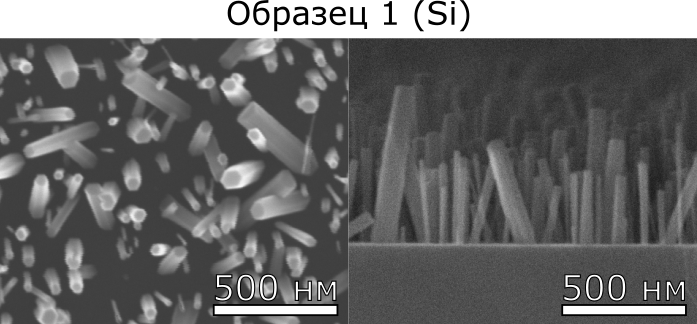
\includegraphics[width=0.45\linewidth]{Image_27_1}}

		\subcaptionbox{\label{fig:Image_27_2}}{%
			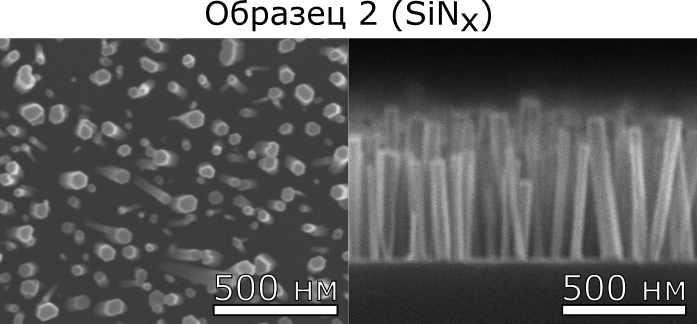
\includegraphics[width=0.45\linewidth]{Image_27_2}}
			\subcaptionbox{\label{fig:Image_27_3}}{%
			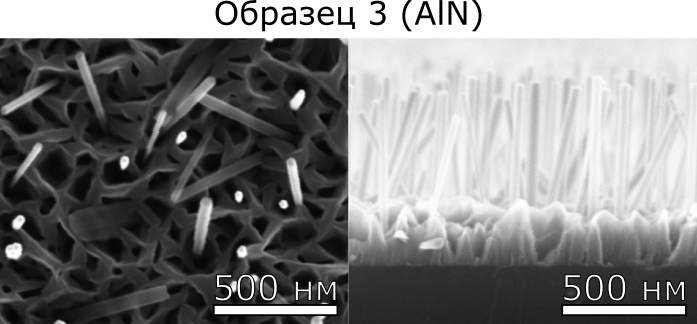
\includegraphics[width=0.45\linewidth]{Image_27_3}}

		\subcaptionbox{\label{fig:Image_27_4}}{%
			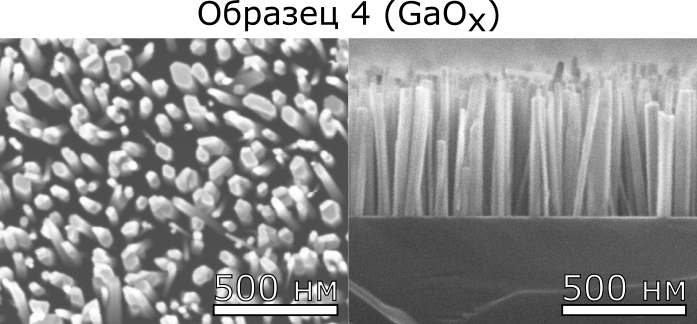
\includegraphics[width=0.45\linewidth]{Image_27_4}}
			\subcaptionbox{\label{fig:Image_27_5}}{%
			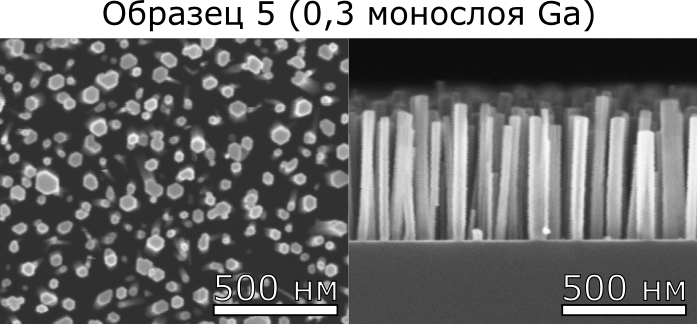
\includegraphics[width=0.45\linewidth]{Image_27_5}}

		\subcaptionbox{\label{fig:Image_27_6}}{%
			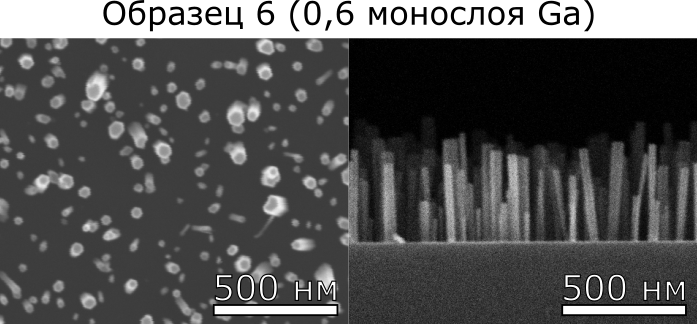
\includegraphics[width=0.45\linewidth]{Image_27_6}}
			\subcaptionbox{\label{fig:Image_27_7}}{%
			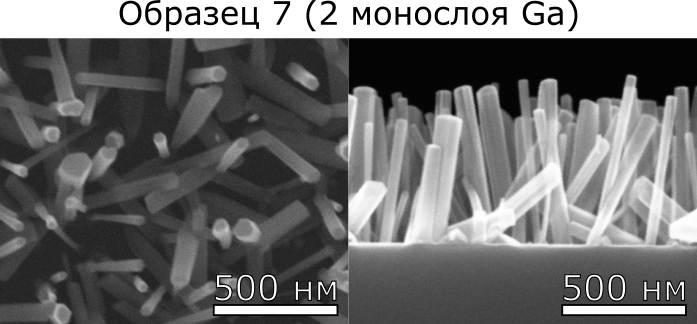
\includegraphics[width=0.45\linewidth]{Image_27_7}} }
			\legend{а)Образец~1: ННК, выращенные на Si, б) образец~2: на SiN, в)
				образец~3: на AlN, г) образец~4: на GaO\textsubscript{x}, д) образец~5:
				на 0,3~монослоях Ga, е) образец~6: на 0,6~монослоях Ga, ж) образец 7:
				на 2~монослоях Ga} \caption{РЭМ изображения синтезированных массивов
		GaN ННК}\label{fig:Image_27} \end{figure}

Согласно анализу РЭМ изображений, рост на необработанной подложке с
реконструкцией Si\((111)7\)\(\times\)\(7\) (образец 1) приводит к образованию
наименее однородного массива в серии по ориентации направлений роста ННК, а их
распределение осевых скоростей роста имеет самую высокую выборочную дисперсию.
Этот метод обеспечивает низкую по серии среднюю скорость осевого роста ННК
(22~\si{\nano\meter\per\hour}) со средним по серии диаметром
(48~\si{\nano\meter}).

Нитридация подложки перед осаждением GaN (образец~2) приводит к увеличению
поверхностной плотности ННК с 52 до 80~\si{\per\micro\meter\squared},
незначительному увеличению средней скорости осевого роста
(28~\si{\nano\meter\per\hour}), обеспечивает высокую ориентированность
синтезированных ННК.

Рост на буферном слое GaO\textsubscript{x} (образец~4) приводит к образованию
массива ННК с высокой поверхностной плотностью
(111~\si{\per\micro\meter\squared}) и высоким диаметром (65~\si{\nano\meter}),
что делает их перспективными для изготовления антиотражающих покрытий
\cite{Mozharov2015a}.

\begin{figure}[ht] \centerfloat{
		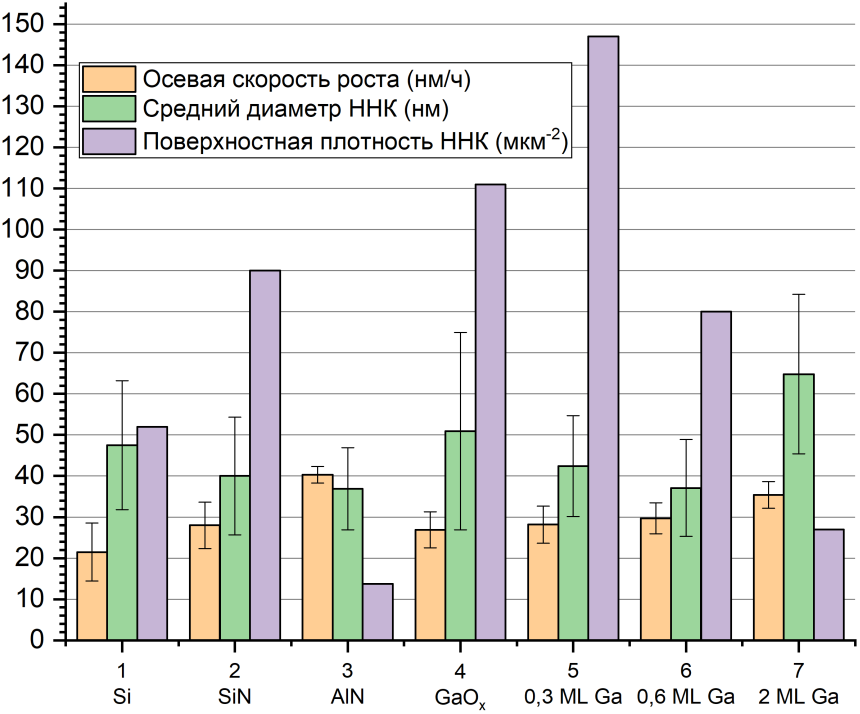
\includegraphics[width=0.7\linewidth]{Image_28} } \caption{Столбчатая
		диаграмма средней (по времени роста) осевой скорости роста, средних (по
		длине ННК) диаметров и поверхностной плотности массивов ННК GaN в
зависимости от метода обработки подложки}\label{fig:Image_28} \end{figure}

Использование смачивающего слоя Ga эквивалентной толщиной 0,3 и 0,6~монослоя
(образцы~5 и~6), нанесенного до нитридации Si, потенциально позволяет добиться
прямой гетерограницы GaN/Si. Анализ экспериментальных данных показывает, что
увеличение толщины слоя Ga приводит к снижению поверхностной плотности с 134 до
65~\si{\per\micro\meter\squared} (0,3~монослоя Ga и 0,6~монослоя Ga
соответственно).

Использование затравочного слоя Ga эквивалентной толщиной в 2 монослоя
значительно снижает поверхностную плотность ННК до
27~\si{\per\micro\meter\squared}, увеличивает средний диаметр
(65~\si{\nano\meter}) и скорость осевого роста (35~\si{\nano\meter\per\hour}).
Выращенные данным способом ННК обладают низкой ориентированностью, что
ограничивает их приборное применение.

Массив ННК, синтезированный на затравке AlN (образец~3) имеет наименьшую
поверхностную плотность (14~\si{\per\micro\meter\squared}) и наибольшую среднюю
скорость осевого роста ННК (40~\si{\nano\meter\per\hour}) с наименьшей
выборочной дисперсией её распределения.

\section{Картина ДБЭ во время роста}\label{sec:ch4/sec3}

Полученные изображения картин ДБЭ для различных азимутальных направлений в
конце роста ННК представлены на~рис.~\cref{fig:Image_29}. Наблюдаемые картины
ДБЭ от ННК соответствуют кристаллической структуре WZ. В работе
\cite{Wierzbicka2013} отмечается сохранение следующих эпитаксиальных отношений
для ННК GaN на Si:
(0001)\textsubscript{GaN}\(\parallel\)(111)\textsubscript{Si} и
<\(112\overline{0}\)>\textsubscript{GaN}\(\parallel\)<\(11\overline{0}\)>\textsubscript{Si}.
На изображениях ДБЭ (см.~рис.~\cref{fig:Image_29}) наблюдается различное
распределения эпитаксиальных ориентаций в зависимости от метода подготовки
поверхности подложки. Наклон ННК наблюдается на РЭМ изображениях ННК GaN,
выращенных на необработанном Si (см.~рис.~\cref{fig:Image_29_1}) и
предварительно нитридированном Si (см.~рис.~\cref{fig:Image_27_2}). Наиболее
низкая дисперсия распределения углов наклона ННК наблюдается на образце с
затравкой AlN (образец~3 (см.~рис.~\cref{fig:Image_27_3})). На образце~7
(2~монослоя Ga) (см.~рис.~\cref{fig:Image_27_7}) присутствуют случайно
наклонённые ННК на угол до 60{\textdegree} к нормали подложки. Это
соответствует наклону оси <0001>\textsubscript{GaN}, который отражается на
картинах ДБЭ поперечным уширением штрихов брэгговских рефлексов.

\begin{figure}[ht] \centerfloat{ \subcaptionbox{\label{fig:Image_29_1}}{%
			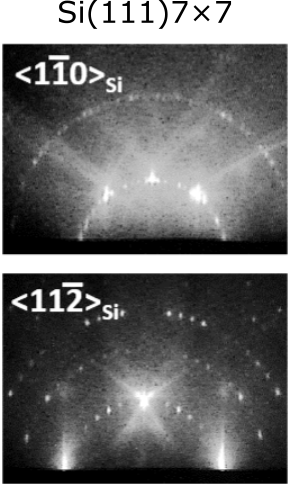
\includegraphics[width=0.2\linewidth]{Image_29_1}}
			\subcaptionbox{\label{fig:Image_29_2}}{%
				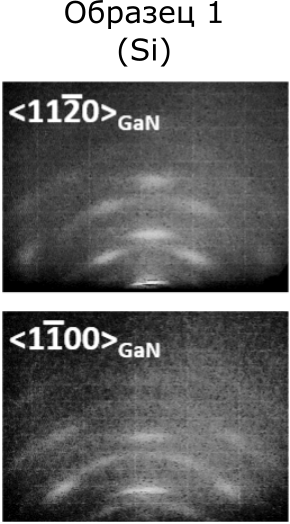
\includegraphics[width=0.2\linewidth]{Image_29_2}}
				\subcaptionbox{\label{fig:Image_29_3}}{%
					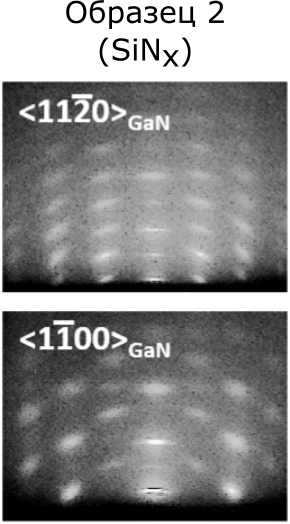
\includegraphics[width=0.2\linewidth]{Image_29_3}}
					\subcaptionbox{\label{fig:Image_29_4}}{%
					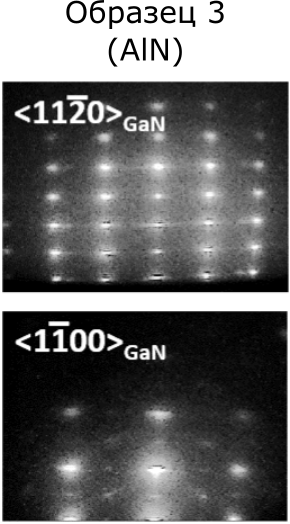
\includegraphics[width=0.2\linewidth]{Image_29_4}}

		\subcaptionbox{\label{fig:Image_29_5}}{%
			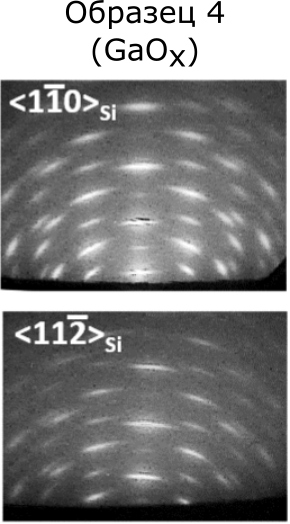
\includegraphics[width=0.2\linewidth]{Image_29_5}}
			\subcaptionbox{\label{fig:Image_29_6}}{%
				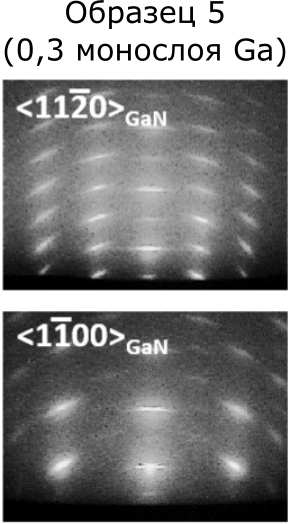
\includegraphics[width=0.2\linewidth]{Image_29_6}}
				\subcaptionbox{\label{fig:Image_29_7}}{%
				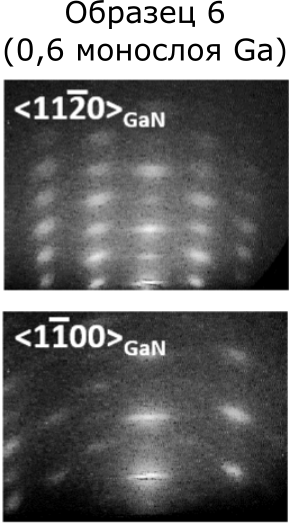
\includegraphics[width=0.2\linewidth]{Image_29_7}}
				\subcaptionbox{\label{fig:Image_29_8}}{%
				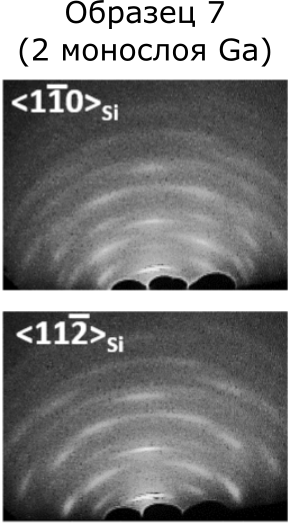
\includegraphics[width=0.2\linewidth]{Image_29_8}} } \legend{Картины
				ДБЭ сняты в направлениях  <\(1\overline{1}0\)>\textsubscript{Si} и
				<\(11\overline{2}\)>\textsubscript{Si}} \caption{Картины ДБЭ
				Si\((111)7\)\(\times\)\(7\), полученные до роста ННК GaN~(а) и в конце
				роста ННК на различных подготовленных поверхностях~(б --
		и)}\label{fig:Image_29} \end{figure}

Поперечное уширения брэгговских рефлексов не наблюдалось для образца~3 (AlN)
(см.~рис.~\cref{fig:Image_29_4}). Как видно из соответствующих РЭМ изображений
(см.~рис.~\cref{fig:Image_27_3}), на этом образце наблюдается паразитное
образование сплошного слоя GaN, образованного сеткой наностен. Это явление
связано с влиянием затравочных островков AlN на зарождение и полярность GaN
\cite{Zhong2018}. Можно предположить, что низкая поверхностная плотность
массива ННК приводит к преобладанию дифракции от сетки наностен при
формировании картины ДБЭ.

За исключением образца~3 (AlN), наиболее четкая картина ДБЭ наблюдается от
массива образца~5 (0.3 монослоя Ga), что свидетельствует о его высоком
кристаллическом совершенстве (см.~рис.~\cref{fig:Image_29_6}). Наиболее
уширенные рефлексы ДБЭ наблюдаются от массива образца~1 (без дополнительной
обработки), что указывает на наклон и несогласованность кристаллической
ориентации ННК в плоскости подложки.

Картина ДБЭ массива образца~4 (GaO\textsubscript{x})
(см.~рис.~\cref{fig:Image_29_5}) полностью независима от азимутальной
ориентации образца, что указывает на мозаичный разброс кристаллографической
ориентации ННК в плоскости подложки, вызванный микрокристалличностью затравки
GaO\textsubscript{x}.

Отклонение и разброс кристаллических ориентаций ННК в плоскости подложки
наблюдаются в массиве образца~7, выращенном на затравке нитридированных капель
Ga эквивалентной толщиной в 2 монослоя (см.~рис.~\cref{fig:Image_27_7}). В
главе~\cref{ch:ch3} обсуждалась нитридация Ga капель и тот факт, что она может
привести к образованию наночастиц ZB-GaN с \{111\}\textsubscript{GaN} гранями,
действующими в качестве центров зародышеобразования для роста ННК
\cite{Fedorov2018}. В этом случае ориентация решётки ННК зависит от
кристаллического качества и ориентации затравок ZB-GaN. Картины ДБЭ от массива
данного образца, снятые вдоль перпендикулярных направлений
<\(1\overline{1}0\)>\textsubscript{Si} и <\(11\overline{2}\)>\textsubscript{Si}
(см.~рис.~\cref{fig:Image_29_8}) схожи, а полукруглое удлинение рефлексов ДБЭ
указывает на высокую мозаичность кристаллографических ориентаций ННК в
плоскости подложки.

\section{Влияние подготовки поверхности на низкотемпературную
ФЛ}\label{sec:ch4/sec4}

На~рис.~\cref{fig:Image_30_1} приведены спектры ФЛ, полученные при температуре
5~\si{\kelvin} с использованием гелиевого криостата с замкнутым циклом. В
спектрах не наблюдается характерной жёлтой линии ФЛ, связанной с высокой
плотностью дефектных состояний \cite{Suski1995}. Все образцы имеют две основные
линий ФЛ с энергиями \(\approx 3,468\)~\si{\electronvolt} и \(\approx
3,472\)~\si{\electronvolt} (обозначены на~рис.~\cref{fig:Image_30_1} линиями a
и b), соответствующие рекомбинации экситонов, связанных на нейтральных донорах
(D\textsubscript{0}~X) (donor bound exciton, DBE) \cite{Bolshakov2018,
Paskov2004}. Полуширина линий \(\approx 4,5\)~\si{\milli\electronvolt} не
позволяет разрешить пики от рекомбинации экситонов на легирующих примесях
кислорода (O\textsuperscript{0},~X\textsuperscript{A}) и кремния
(Si\textsuperscript{0},~X\textsuperscript{A}) \cite{Zettler2015}, однако стоит
полагать, что (Si\textsuperscript{0},~X\textsuperscript{A}) переходы вносят
больший вклад в сигнал ФЛ из-за преднамеренного Si легирования в течение
последних нескольких часов роста до концентрации
10\textsuperscript{19}~\si{\per\centi\metre\cubed}. В данной работе не
исследовалось пространственное распределение легирующей примеси, однако, нижняя
часть ННК также может быть легирована Si из-за радиального роста и объёмной
диффузии атомов Si на гетерогранице с кремниевой подложкой. По этим причинам
экситоны, связанные на акцепторе, в исследуемых образцах не ожидаются.
Появление линий a и b может быть вызвано донорно связанными тяжело-
(D\textsuperscript{0},~X\textsuperscript{B}) и лёгкодырочными
(D\textsuperscript{0},~X\textsuperscript{A}) экситонными переходами. Другая
возможная причина расщепления DBE связана с поверхностными эффектами
\cite{Calarco2011}, влияющими на энергию связи экситон\,--\,донор или
вызывающими неоднородность концентрации легирующей примеси, так как излучение
DBE может испытывать красное смещение на \(\approx 6\)~\si{\milli\electronvolt}
при увеличении концентрации легирующей примеси Si на порядок (c
10\textsuperscript{17} до 10\textsuperscript{18}~\si{\per\centi\metre\cubed})
\cite{Pozina2011}.

\begin{figure}[ht] \centerfloat{
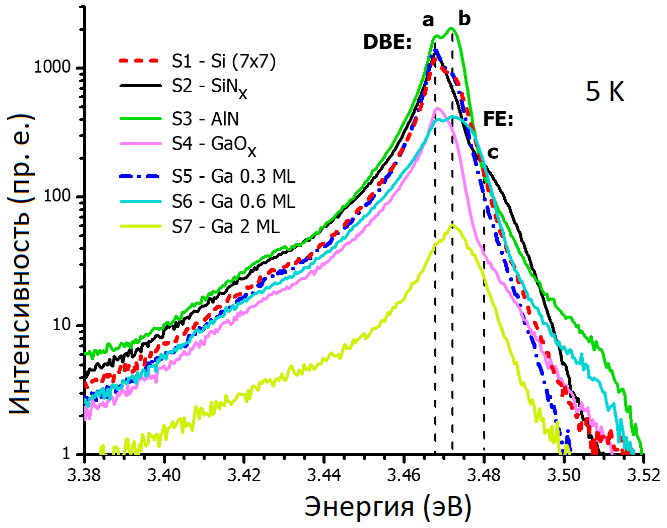
\includegraphics[width=0.6\linewidth]{Image_30_1} } \caption{Низкотемпературные
спектры ФЛ синтезированных массивов ННК GaN}\label{fig:Image_30_1} \end{figure}

Высокоэнергетическое плечо спектра ФЛ (линия c на~рис.~\cref{fig:Image_30_1})
может быть связано с рекомбинацией экситонов со свободной дыркой
(X\textsuperscript{A},~X\textsuperscript{B}) (free hole exciton, FE).

Спектры ФЛ имеют различную интенсивность и ширину линий в зависимости от метода
подготовки ростовой поверхности, что может быть вызвано структурными
нарушениями, различием в морфологии массивов ННК. Низкая интенсивность ФЛ от
массивов образца~4 (GaO\textsubscript{x}) и образца~6 (0,6~монослоя Ga) может
быть связана с многочисленным слиянием ННК, и вызванными им протяжёнными
дефектами упаковки, что подтверждается уширением рефлексов на картинах ДБЭ.
Наименьшую интенсивность сигнала ФЛ имеет массив образца~7 (2~монослоя Ga).
Остальные образцы (за исключением образца~3 (AlN)) имеют близкие интенсивности
ФЛ. Спектр ФЛ от массива образца~2 (SiN) имеет наиболее интенсивную
коротковолновую линию c и слабую DBE линию b. Такое различие может быть вызвано
низким уровнем легирования, так как нитридация поверхности подложки может
препятствовать объёмной диффузии Si из подложки в растущий ННК. Образец~1 и
образец~5 (0,3~монослоя Ga) имеют схожую форму спектра ФЛ и близкое отношение
интенсивностей линий a/b, аналогично образцу~4 (GaO\textsubscript{x}), однако
он может иметь отличный механизм ФЛ из-за непреднамеренного легирования
кислородом.

Наибольшая интенсивность ФЛ была получена от образца~3 (AlN): низкая
поверхностная плотность позволяет избежать слияния ННК и связанных с ним
структурных дефектов, что уменьшает вероятность безызлучательной рекомбинации и
позволяет добиться высокой интенсивности сигнала ФЛ. Спектр ФЛ обладает низким
отношениями интенсивностей a/b-линий. ННК массива обладают аналогичными
поперечными размерами и самой высокой скоростью осевого роста среди образцов,
что при постоянном потоке Si легирующей примеси приводит к меньшей объёмной
концентрации доноров. Как видно на РЭМ изображениях
(см.~рис.~\cref{fig:Image_27_3}), на подложке Si присутствует слой объёмного
материала сетки наностен GaN высотой 200~\si{\nano\meter}. В данный слой также
встраиваются адатомы легирующей примеси, что значительно снижает уровень
легирования и может объяснить различие в сигнале ФЛ. Чтобы удалить ННК с
подложки (см. вставку на~рис.~\cref{fig:Image_30_2}) и изучить вклад объёмного
слоя в интенсивность ФЛ поверхность подложки была механически процарапана с
последующей обработкой образца в ультразвуковой ванне. Проведено
низкотемпературное исследование ФЛ (10~\si{\kelvin}) исходного образца и
образца после удаления массива ННК (см.~рис.~\cref{fig:Image_30_2}). Измерение
проводилось за один подход, чтобы обеспечить достоверное сравнение.
Интенсивность ФЛ после удаления ННК составляет \(\approx 40\,\%\) от
первоначальной. Можно предположить, что планарные слои GaN, выращенные на
подложке Si, имеют низкую эффективность ФЛ из-за безызлучательной рекомбинацией
на дефектах, вызванных рассогласованием решёток \cite{Calleja1999,
Reshchikov2005}.

\begin{figure}[ht] \centerfloat{
		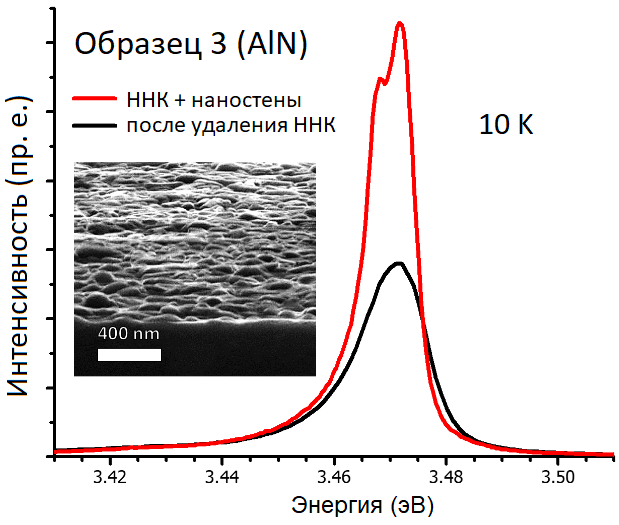
\includegraphics[width=0.6\linewidth]{Image_30_2} } \legend{На вставке РЭМ
		изображение образца~3 (AlN) после удаления ННК, масштабная метка
		400~\si{\nano\meter}} \caption{Низкотемпературные спектры ФЛ образца 3
		(AlN), полученные до (красная кривая) и после (чёрная кривая) удаления
ННК}\label{fig:Image_30_2} \end{figure}

\section{Обсуждение экспериментальных данных}\label{sec:ch4/sec5}

Высокая дисперсия средней по времени осевой скорости роста и низкая
ориентированность ННК массива образца~1 обусловлена поверхностной
неоднородностью из-за нитридации Si, которая начинается одновременно с ростом
GaN и продолжается во время роста.

В случае с AlN затравкой, зарождение ННК GaN неоднородно по поверхности и
обусловлено наличием N-полярных островков AlN. Наряду с этим Ga-полярная сетка
GaN наностен покрывает Al-полярный слой AlN, который занимает большую долю
поверхности образца \cite{Auzelle2015}. Формирование AlN затравки путём
нитридации Al капель на высоких температурах может привести к дополнительной
поверхностной неоднородности, вызванной локальным легированием подложки из-за
растворимости Al в Si. Самая высокая скорость осевого роста ННК GaN на затравке
AlN и самая высокая интенсивность ФЛ среди всех исследованных методов делают
данный ростовой метод привлекательным для создания оптоэлектронных устройств.

Использование затравочного слоя нанокапель Ga эквивалентной толщиной 2 монослоя
приводит к росту однородных по длине наклонных ННК. В главе~\cref{ch:ch3} было
показано, что нитридация капель Ga приводит к образованию наноостровков ZB-GaN
с кристаллографической ориентацией
(111)\textsubscript{ZB-GaN}\(\parallel\)(111)\textsubscript{Si} или
(001)\textsubscript{ZB-GaN}\(\parallel\)(111)\textsubscript{Si}
\cite{Fedorov2018}. Предполагается, что образующиеся наноостровки огранены
плоскостями \{111\}\textsubscript{ZB-GaN}, которые могут выступать в качестве
центров зарождения для роста наклонных ветвей WZ-GaN. Неоднородность ориентаций
ННК определяется подготовкой наноостровков: размером и поверхностной плотностью
капель Ga, условиями нитридации. В неоптимальных условиях роста может
происходить двойникование (вращение на 180{\textdegree} вокруг всех возможных
направлений <111>) кристаллической решётки наночастиц ZB-GaN, приводящее к
случайной ориентации их граней \{111\}\textsubscript{ZB-GaN} и, следовательно,
случайной ориентации зародившихся на этих гранях ННК. Данный образец имеет
наименьшую интенсивность сигнала ФЛ из-за наличия дефектов при слиянии
наклонных ННК.

В случае однородной поверхности роста коэффициент вариации размеров ННК и
скорость роста в основном определяются диффузией и десорбцией адатомов. Поэтому
формирование вертикальных массивов ННК на GaO\textsubscript{x} может быть
объяснено с точки зрения механизма самоиндуцированного роста, обусловленного
анизотропией поверхностных энергий и диффузией адатомов Ga и N, а не влиянием
ориентации подложки или кристаллической структуры \cite{Sobanska2016}.
Поликристалличность GaO\textsubscript{x} приводит к случайной ориентации в
плоскости подложки, а наличие однородной гладкой поверхности
GaO\textsubscript{x} определяет вертикальность массивов GaN ННК.

Морфология массивов ННК, выращенных на нитридированной поверхности
(111)\textsubscript{Si} и поверхности с эквивалентной толщиной Ga в 0,6
монослоя, весьма схожа, а массив на смачивающем слое Ga эквивалентной толщиной
0,3 монослоя имеет поверхностную плотность ННК почти в два раза выше.

\section{Основные результаты}\label{sec:ch4/sec6}

Исследовано эпитаксиальное формирование ННК GaN на обработанной различными
методами подложке Si(111): нитридированной в активированном азоте с
образованием слоя SiN\textsubscript{x}, с буферным слоем GaO\textsubscript{x},
с затравочными островками AlN и GaN, со смачивающими слоями Ga эквивалентной
толщиной 0,3 и 0,6~монослоя. Показано, как подготовка ростовой поверхности
влияет на морфологию и оптические свойства ННК GaN. Наиболее однородный по
длине ННК массив был получен на буферном слое AlN, а наименее однородный массив
получен на необработанной подложке. Вертикальный массив ННК со случайными
кристаллическими ориентациями в плоскости подложки был получен на
микрокристаллическом широкозонном полупроводниковом буферном слое
GaO\textsubscript{x}.

На спектрах ФЛ от синтезированных образцов наблюдается интенсивный сигнал,
обусловленный рекомбинацией экситонов, связанных на нейтральных донорах.
Наибольшая интенсивность ФЛ наблюдается от массива ННК на AlN, а наименьшая~---
от массива на наноостровках GaN, полученных после нитридации капель Ga.

\FloatBarrier
